%% PocketBlock / Barebones 2D Template / mgzy colorway 0.8 / (C) 2016 Justin Troutman

\documentclass[border=1cm]{standalone}

\usepackage{xcolor}
\usepackage{tikz}

\usetikzlibrary{positioning}

\definecolor{pmgzy}{RGB}{47,16,105} % purple
\definecolor{tmgzy}{RGB}{85,168,176} % teal

\begin{document}

\pagecolor{white}

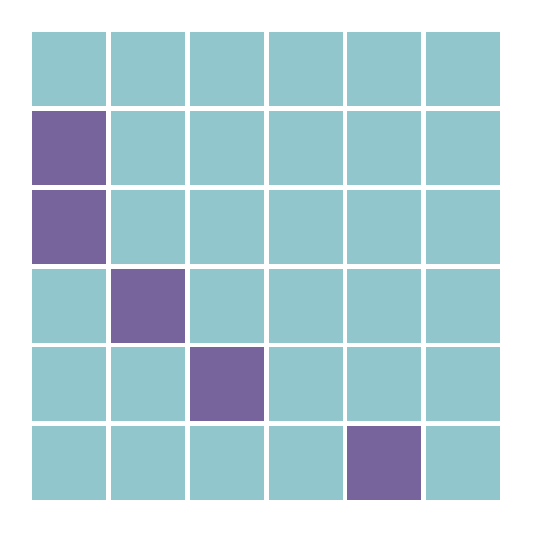
\begin{tikzpicture}[on grid, font=\bfseries, line width=.6mm, line join=bevel]

%% add front face of blocks -- starting from bottom row

%% first row (bottom)
\draw[white, fill=tmgzy!65] (0,0) rectangle (1,1);
\draw[white, fill=tmgzy!65] (1,1) rectangle (2,0);
\draw[white, fill=tmgzy!65] (2,1) rectangle (3,0);
\draw[white, fill=tmgzy!65] (3,1) rectangle (4,0);
\draw[white, fill=pmgzy!65] (4,1) rectangle (5,0);
\draw[white, fill=tmgzy!65] (5,1) rectangle (6,0);

%% second row
\draw[white, fill=tmgzy!65] (0,1) rectangle (1,2);
\draw[white, fill=tmgzy!65] (1,1) rectangle (2,2);
\draw[white, fill=pmgzy!65] (2,1) rectangle (3,2);
\draw[white, fill=tmgzy!65] (3,1) rectangle (4,2);
\draw[white, fill=tmgzy!65] (4,1) rectangle (5,2);
\draw[white, fill=tmgzy!65] (5,1) rectangle (6,2);

%% third row
\draw[white, fill=tmgzy!65]  (0,2) rectangle (1,3);
\draw[white, fill=pmgzy!65]  (1,2) rectangle (2,3);
\draw[white, fill=tmgzy!65]  (2,2) rectangle (3,3);
\draw[white, fill=tmgzy!65]  (3,2) rectangle (4,3);
\draw[white, fill=tmgzy!65]  (4,2) rectangle (5,3);
\draw[white, fill=tmgzy!65]  (5,2) rectangle (6,3);

%% fourth row
\draw[white, fill=pmgzy!65] (0,3) rectangle (1,4);
\draw[white, fill=tmgzy!65] (1,3) rectangle (2,4);
\draw[white, fill=tmgzy!65] (2,3) rectangle (3,4);
\draw[white, fill=tmgzy!65] (3,3) rectangle (4,4);
\draw[white, fill=tmgzy!65] (4,3) rectangle (5,4);
\draw[white, fill=tmgzy!65] (5,3) rectangle (6,4);

%% fifth row
\draw[white, fill=pmgzy!65] (0,4) rectangle (1,5);
\draw[white, fill=tmgzy!65] (1,4) rectangle (2,5);
\draw[white, fill=tmgzy!65] (2,4) rectangle (3,5);
\draw[white, fill=tmgzy!65] (3,4) rectangle (4,5);
\draw[white, fill=tmgzy!65] (4,4) rectangle (5,5);
\draw[white, fill=tmgzy!65] (5,4) rectangle (6,5);

%% sixth row (top)
\draw[white, fill=tmgzy!65] (0,5) rectangle (1,6);
\draw[white, fill=tmgzy!65] (1,5) rectangle (2,6);
\draw[white, fill=tmgzy!65] (2,5) rectangle (3,6);
\draw[white, fill=tmgzy!65] (3,5) rectangle (4,6); 
\draw[white, fill=tmgzy!65] (4,5) rectangle (5,6); 
\draw[white, fill=tmgzy!65] (5,5) rectangle (6,6); 

\end{tikzpicture}

\end{document}